\section{0110}

\begin{center}
\begin{tabular}{cccc} 
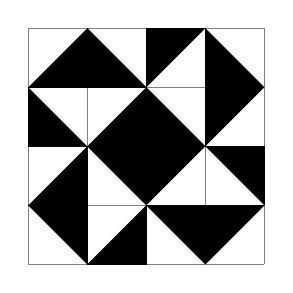
\begin{tikzpicture}[scale=0.75]
 \draw [step=1cm,gray,very thin](0,-1) grid (4,3); 
 \draw[opacity=1,fill=black](0,0)--(1,0)--(1,-1); 
 \draw[opacity=1,fill=black](1,1)--(1,0)--(0,0); 
 \draw[opacity=1,fill=black](1,1)--(0,1)--(0,2); 
 \draw[opacity=1,fill=black](1,3)--(1,2)--(0,2); 
 \draw[opacity=1,fill=black](2,0)--(2,-1)--(1,-1); 
 \draw[opacity=1,fill=black](1,1)--(2,1)--(2,0); 
 \draw[opacity=1,fill=black](2,2)--(2,1)--(1,1); 
 \draw[opacity=1,fill=black](2,2)--(1,2)--(1,3); 
 \draw[opacity=1,fill=black](2,0)--(3,0)--(3,-1); 
 \draw[opacity=1,fill=black](2,0)--(2,1)--(3,1); 
 \draw[opacity=1,fill=black](3,1)--(2,1)--(2,2); 
 \draw[opacity=1,fill=black](2,2)--(2,3)--(3,3); 
 \draw[opacity=1,fill=black](3,-1)--(3,0)--(4,0); 
 \draw[opacity=1,fill=black](3,1)--(4,1)--(4,0); 
 \draw[opacity=1,fill=black](3,1)--(3,2)--(4,2); 
 \draw[opacity=1,fill=black](4,2)--(3,2)--(3,3); 
\end{tikzpicture} 
 & 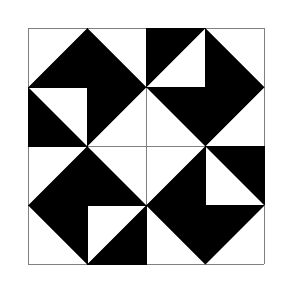
\begin{tikzpicture}[scale=0.75]
 \draw [step=1cm,gray,very thin](0,-1) grid (4,3); 
 \draw[opacity=1,fill=black](0,0)--(1,0)--(1,-1); 
 \draw[opacity=1,fill=black](1,1)--(1,0)--(0,0); 
 \draw[opacity=1,fill=black](1,1)--(0,1)--(0,2); 
 \draw[opacity=1,fill=black](1,3)--(1,2)--(0,2); 
 \draw[opacity=1,fill=black](2,0)--(2,-1)--(1,-1); 
 \draw[opacity=1,fill=black](2,0)--(1,0)--(1,1); 
 \draw[opacity=1,fill=black](1,1)--(1,2)--(2,2); 
 \draw[opacity=1,fill=black](2,2)--(1,2)--(1,3); 
 \draw[opacity=1,fill=black](2,0)--(3,0)--(3,-1); 
 \draw[opacity=1,fill=black](3,1)--(3,0)--(2,0); 
 \draw[opacity=1,fill=black](2,2)--(3,2)--(3,1); 
 \draw[opacity=1,fill=black](2,2)--(2,3)--(3,3); 
 \draw[opacity=1,fill=black](3,-1)--(3,0)--(4,0); 
 \draw[opacity=1,fill=black](3,1)--(4,1)--(4,0); 
 \draw[opacity=1,fill=black](3,1)--(3,2)--(4,2); 
 \draw[opacity=1,fill=black](4,2)--(3,2)--(3,3); 
\end{tikzpicture} 
 & 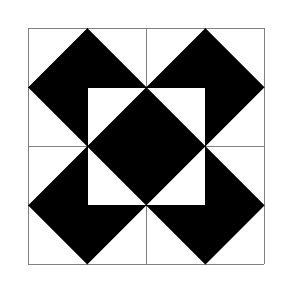
\begin{tikzpicture}[scale=0.75]
 \draw [step=1cm,gray,very thin](0,-1) grid (4,3); 
 \draw[opacity=1,fill=black](0,0)--(1,0)--(1,-1); 
 \draw[opacity=1,fill=black](1,1)--(1,0)--(0,0); 
 \draw[opacity=1,fill=black](0,2)--(1,2)--(1,1); 
 \draw[opacity=1,fill=black](1,3)--(1,2)--(0,2); 
 \draw[opacity=1,fill=black](1,-1)--(1,0)--(2,0); 
 \draw[opacity=1,fill=black](1,1)--(2,1)--(2,0); 
 \draw[opacity=1,fill=black](2,2)--(2,1)--(1,1); 
 \draw[opacity=1,fill=black](2,2)--(1,2)--(1,3); 
 \draw[opacity=1,fill=black](2,0)--(3,0)--(3,-1); 
 \draw[opacity=1,fill=black](2,0)--(2,1)--(3,1); 
 \draw[opacity=1,fill=black](3,1)--(2,1)--(2,2); 
 \draw[opacity=1,fill=black](3,3)--(3,2)--(2,2); 
 \draw[opacity=1,fill=black](3,-1)--(3,0)--(4,0); 
 \draw[opacity=1,fill=black](4,0)--(3,0)--(3,1); 
 \draw[opacity=1,fill=black](3,1)--(3,2)--(4,2); 
 \draw[opacity=1,fill=black](4,2)--(3,2)--(3,3); 
\end{tikzpicture} 
 & 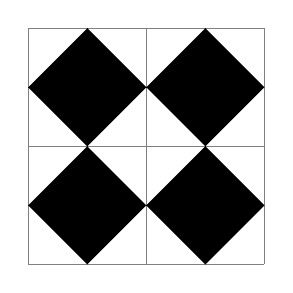
\begin{tikzpicture}[scale=0.75]
 \draw [step=1cm,gray,very thin](0,-1) grid (4,3); 
 \draw[opacity=1,fill=black](0,0)--(1,0)--(1,-1); 
 \draw[opacity=1,fill=black](1,1)--(1,0)--(0,0); 
 \draw[opacity=1,fill=black](0,2)--(1,2)--(1,1); 
 \draw[opacity=1,fill=black](1,3)--(1,2)--(0,2); 
 \draw[opacity=1,fill=black](1,-1)--(1,0)--(2,0); 
 \draw[opacity=1,fill=black](2,0)--(1,0)--(1,1); 
 \draw[opacity=1,fill=black](1,1)--(1,2)--(2,2); 
 \draw[opacity=1,fill=black](2,2)--(1,2)--(1,3); 
 \draw[opacity=1,fill=black](2,0)--(3,0)--(3,-1); 
 \draw[opacity=1,fill=black](3,1)--(3,0)--(2,0); 
 \draw[opacity=1,fill=black](2,2)--(3,2)--(3,1); 
 \draw[opacity=1,fill=black](3,3)--(3,2)--(2,2); 
 \draw[opacity=1,fill=black](3,-1)--(3,0)--(4,0); 
 \draw[opacity=1,fill=black](4,0)--(3,0)--(3,1); 
 \draw[opacity=1,fill=black](3,1)--(3,2)--(4,2); 
 \draw[opacity=1,fill=black](4,2)--(3,2)--(3,3); 
\end{tikzpicture} 
\\ 
 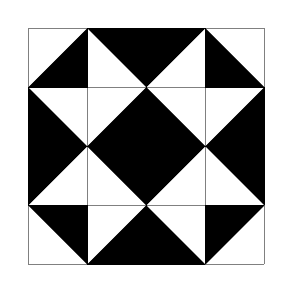
\begin{tikzpicture}[scale=0.75]
 \draw [step=1cm,gray,very thin](0,-1) grid (4,3); 
 \draw[opacity=1,fill=black](0,0)--(1,0)--(1,-1); 
 \draw[opacity=1,fill=black](0,0)--(0,1)--(1,1); 
 \draw[opacity=1,fill=black](1,1)--(0,1)--(0,2); 
 \draw[opacity=1,fill=black](1,3)--(1,2)--(0,2); 
 \draw[opacity=1,fill=black](2,0)--(2,-1)--(1,-1); 
 \draw[opacity=1,fill=black](1,1)--(2,1)--(2,0); 
 \draw[opacity=1,fill=black](2,2)--(2,1)--(1,1); 
 \draw[opacity=1,fill=black](1,3)--(2,3)--(2,2); 
 \draw[opacity=1,fill=black](3,-1)--(2,-1)--(2,0); 
 \draw[opacity=1,fill=black](2,0)--(2,1)--(3,1); 
 \draw[opacity=1,fill=black](3,1)--(2,1)--(2,2); 
 \draw[opacity=1,fill=black](2,2)--(2,3)--(3,3); 
 \draw[opacity=1,fill=black](3,-1)--(3,0)--(4,0); 
 \draw[opacity=1,fill=black](3,1)--(4,1)--(4,0); 
 \draw[opacity=1,fill=black](4,2)--(4,1)--(3,1); 
 \draw[opacity=1,fill=black](4,2)--(3,2)--(3,3); 
\end{tikzpicture} 
 & 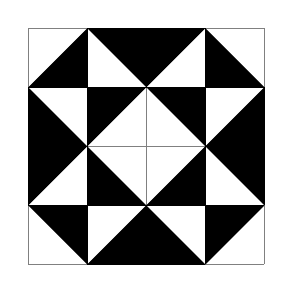
\begin{tikzpicture}[scale=0.75]
 \draw [step=1cm,gray,very thin](0,-1) grid (4,3); 
 \draw[opacity=1,fill=black](0,0)--(1,0)--(1,-1); 
 \draw[opacity=1,fill=black](0,0)--(0,1)--(1,1); 
 \draw[opacity=1,fill=black](1,1)--(0,1)--(0,2); 
 \draw[opacity=1,fill=black](1,3)--(1,2)--(0,2); 
 \draw[opacity=1,fill=black](2,0)--(2,-1)--(1,-1); 
 \draw[opacity=1,fill=black](2,0)--(1,0)--(1,1); 
 \draw[opacity=1,fill=black](1,1)--(1,2)--(2,2); 
 \draw[opacity=1,fill=black](1,3)--(2,3)--(2,2); 
 \draw[opacity=1,fill=black](3,-1)--(2,-1)--(2,0); 
 \draw[opacity=1,fill=black](3,1)--(3,0)--(2,0); 
 \draw[opacity=1,fill=black](2,2)--(3,2)--(3,1); 
 \draw[opacity=1,fill=black](2,2)--(2,3)--(3,3); 
 \draw[opacity=1,fill=black](3,-1)--(3,0)--(4,0); 
 \draw[opacity=1,fill=black](3,1)--(4,1)--(4,0); 
 \draw[opacity=1,fill=black](4,2)--(4,1)--(3,1); 
 \draw[opacity=1,fill=black](4,2)--(3,2)--(3,3); 
\end{tikzpicture} 
 & 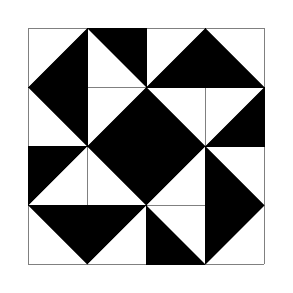
\begin{tikzpicture}[scale=0.75]
 \draw [step=1cm,gray,very thin](0,-1) grid (4,3); 
 \draw[opacity=1,fill=black](0,0)--(1,0)--(1,-1); 
 \draw[opacity=1,fill=black](0,0)--(0,1)--(1,1); 
 \draw[opacity=1,fill=black](0,2)--(1,2)--(1,1); 
 \draw[opacity=1,fill=black](1,3)--(1,2)--(0,2); 
 \draw[opacity=1,fill=black](1,-1)--(1,0)--(2,0); 
 \draw[opacity=1,fill=black](1,1)--(2,1)--(2,0); 
 \draw[opacity=1,fill=black](2,2)--(2,1)--(1,1); 
 \draw[opacity=1,fill=black](1,3)--(2,3)--(2,2); 
 \draw[opacity=1,fill=black](3,-1)--(2,-1)--(2,0); 
 \draw[opacity=1,fill=black](2,0)--(2,1)--(3,1); 
 \draw[opacity=1,fill=black](3,1)--(2,1)--(2,2); 
 \draw[opacity=1,fill=black](3,3)--(3,2)--(2,2); 
 \draw[opacity=1,fill=black](3,-1)--(3,0)--(4,0); 
 \draw[opacity=1,fill=black](4,0)--(3,0)--(3,1); 
 \draw[opacity=1,fill=black](4,2)--(4,1)--(3,1); 
 \draw[opacity=1,fill=black](4,2)--(3,2)--(3,3); 
\end{tikzpicture} 
 & 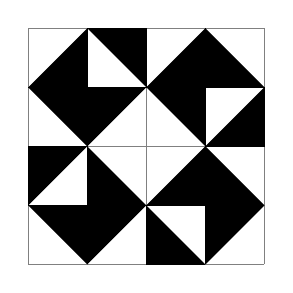
\begin{tikzpicture}[scale=0.75]
 \draw [step=1cm,gray,very thin](0,-1) grid (4,3); 
 \draw[opacity=1,fill=black](0,0)--(1,0)--(1,-1); 
 \draw[opacity=1,fill=black](0,0)--(0,1)--(1,1); 
 \draw[opacity=1,fill=black](0,2)--(1,2)--(1,1); 
 \draw[opacity=1,fill=black](1,3)--(1,2)--(0,2); 
 \draw[opacity=1,fill=black](1,-1)--(1,0)--(2,0); 
 \draw[opacity=1,fill=black](2,0)--(1,0)--(1,1); 
 \draw[opacity=1,fill=black](1,1)--(1,2)--(2,2); 
 \draw[opacity=1,fill=black](1,3)--(2,3)--(2,2); 
 \draw[opacity=1,fill=black](3,-1)--(2,-1)--(2,0); 
 \draw[opacity=1,fill=black](3,1)--(3,0)--(2,0); 
 \draw[opacity=1,fill=black](2,2)--(3,2)--(3,1); 
 \draw[opacity=1,fill=black](3,3)--(3,2)--(2,2); 
 \draw[opacity=1,fill=black](3,-1)--(3,0)--(4,0); 
 \draw[opacity=1,fill=black](4,0)--(3,0)--(3,1); 
 \draw[opacity=1,fill=black](4,2)--(4,1)--(3,1); 
 \draw[opacity=1,fill=black](4,2)--(3,2)--(3,3); 
\end{tikzpicture} 
\\ 
 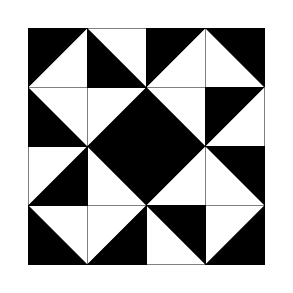
\begin{tikzpicture}[scale=0.75]
 \draw [step=1cm,gray,very thin](0,-1) grid (4,3); 
 \draw[opacity=1,fill=black](1,-1)--(0,-1)--(0,0); 
 \draw[opacity=1,fill=black](1,1)--(1,0)--(0,0); 
 \draw[opacity=1,fill=black](1,1)--(0,1)--(0,2); 
 \draw[opacity=1,fill=black](0,2)--(0,3)--(1,3); 
 \draw[opacity=1,fill=black](2,0)--(2,-1)--(1,-1); 
 \draw[opacity=1,fill=black](1,1)--(2,1)--(2,0); 
 \draw[opacity=1,fill=black](2,2)--(2,1)--(1,1); 
 \draw[opacity=1,fill=black](2,2)--(1,2)--(1,3); 
 \draw[opacity=1,fill=black](2,0)--(3,0)--(3,-1); 
 \draw[opacity=1,fill=black](2,0)--(2,1)--(3,1); 
 \draw[opacity=1,fill=black](3,1)--(2,1)--(2,2); 
 \draw[opacity=1,fill=black](2,2)--(2,3)--(3,3); 
 \draw[opacity=1,fill=black](4,0)--(4,-1)--(3,-1); 
 \draw[opacity=1,fill=black](3,1)--(4,1)--(4,0); 
 \draw[opacity=1,fill=black](3,1)--(3,2)--(4,2); 
 \draw[opacity=1,fill=black](3,3)--(4,3)--(4,2); 
\end{tikzpicture} 
 & 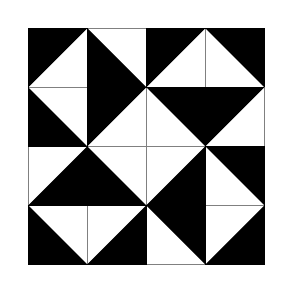
\begin{tikzpicture}[scale=0.75]
 \draw [step=1cm,gray,very thin](0,-1) grid (4,3); 
 \draw[opacity=1,fill=black](1,-1)--(0,-1)--(0,0); 
 \draw[opacity=1,fill=black](1,1)--(1,0)--(0,0); 
 \draw[opacity=1,fill=black](1,1)--(0,1)--(0,2); 
 \draw[opacity=1,fill=black](0,2)--(0,3)--(1,3); 
 \draw[opacity=1,fill=black](2,0)--(2,-1)--(1,-1); 
 \draw[opacity=1,fill=black](2,0)--(1,0)--(1,1); 
 \draw[opacity=1,fill=black](1,1)--(1,2)--(2,2); 
 \draw[opacity=1,fill=black](2,2)--(1,2)--(1,3); 
 \draw[opacity=1,fill=black](2,0)--(3,0)--(3,-1); 
 \draw[opacity=1,fill=black](3,1)--(3,0)--(2,0); 
 \draw[opacity=1,fill=black](2,2)--(3,2)--(3,1); 
 \draw[opacity=1,fill=black](2,2)--(2,3)--(3,3); 
 \draw[opacity=1,fill=black](4,0)--(4,-1)--(3,-1); 
 \draw[opacity=1,fill=black](3,1)--(4,1)--(4,0); 
 \draw[opacity=1,fill=black](3,1)--(3,2)--(4,2); 
 \draw[opacity=1,fill=black](3,3)--(4,3)--(4,2); 
\end{tikzpicture} 
 & 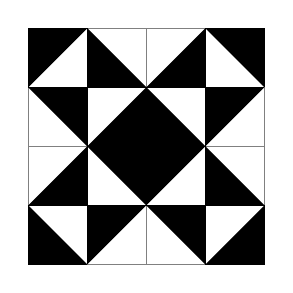
\begin{tikzpicture}[scale=0.75]
 \draw [step=1cm,gray,very thin](0,-1) grid (4,3); 
 \draw[opacity=1,fill=black](1,-1)--(0,-1)--(0,0); 
 \draw[opacity=1,fill=black](1,1)--(1,0)--(0,0); 
 \draw[opacity=1,fill=black](0,2)--(1,2)--(1,1); 
 \draw[opacity=1,fill=black](0,2)--(0,3)--(1,3); 
 \draw[opacity=1,fill=black](1,-1)--(1,0)--(2,0); 
 \draw[opacity=1,fill=black](1,1)--(2,1)--(2,0); 
 \draw[opacity=1,fill=black](2,2)--(2,1)--(1,1); 
 \draw[opacity=1,fill=black](2,2)--(1,2)--(1,3); 
 \draw[opacity=1,fill=black](2,0)--(3,0)--(3,-1); 
 \draw[opacity=1,fill=black](2,0)--(2,1)--(3,1); 
 \draw[opacity=1,fill=black](3,1)--(2,1)--(2,2); 
 \draw[opacity=1,fill=black](3,3)--(3,2)--(2,2); 
 \draw[opacity=1,fill=black](4,0)--(4,-1)--(3,-1); 
 \draw[opacity=1,fill=black](4,0)--(3,0)--(3,1); 
 \draw[opacity=1,fill=black](3,1)--(3,2)--(4,2); 
 \draw[opacity=1,fill=black](3,3)--(4,3)--(4,2); 
\end{tikzpicture} 
 & 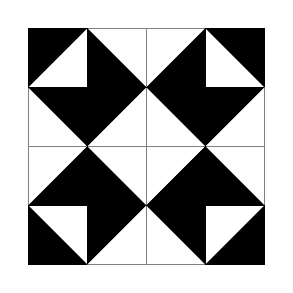
\begin{tikzpicture}[scale=0.75]
 \draw [step=1cm,gray,very thin](0,-1) grid (4,3); 
 \draw[opacity=1,fill=black](1,-1)--(0,-1)--(0,0); 
 \draw[opacity=1,fill=black](1,1)--(1,0)--(0,0); 
 \draw[opacity=1,fill=black](0,2)--(1,2)--(1,1); 
 \draw[opacity=1,fill=black](0,2)--(0,3)--(1,3); 
 \draw[opacity=1,fill=black](1,-1)--(1,0)--(2,0); 
 \draw[opacity=1,fill=black](2,0)--(1,0)--(1,1); 
 \draw[opacity=1,fill=black](1,1)--(1,2)--(2,2); 
 \draw[opacity=1,fill=black](2,2)--(1,2)--(1,3); 
 \draw[opacity=1,fill=black](2,0)--(3,0)--(3,-1); 
 \draw[opacity=1,fill=black](3,1)--(3,0)--(2,0); 
 \draw[opacity=1,fill=black](2,2)--(3,2)--(3,1); 
 \draw[opacity=1,fill=black](3,3)--(3,2)--(2,2); 
 \draw[opacity=1,fill=black](4,0)--(4,-1)--(3,-1); 
 \draw[opacity=1,fill=black](4,0)--(3,0)--(3,1); 
 \draw[opacity=1,fill=black](3,1)--(3,2)--(4,2); 
 \draw[opacity=1,fill=black](3,3)--(4,3)--(4,2); 
\end{tikzpicture} 
\\ 
 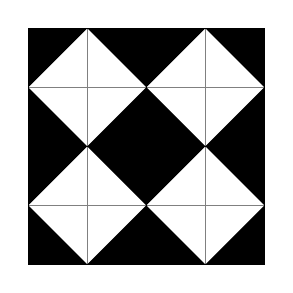
\begin{tikzpicture}[scale=0.75]
 \draw [step=1cm,gray,very thin](0,-1) grid (4,3); 
 \draw[opacity=1,fill=black](1,-1)--(0,-1)--(0,0); 
 \draw[opacity=1,fill=black](0,0)--(0,1)--(1,1); 
 \draw[opacity=1,fill=black](1,1)--(0,1)--(0,2); 
 \draw[opacity=1,fill=black](0,2)--(0,3)--(1,3); 
 \draw[opacity=1,fill=black](2,0)--(2,-1)--(1,-1); 
 \draw[opacity=1,fill=black](1,1)--(2,1)--(2,0); 
 \draw[opacity=1,fill=black](2,2)--(2,1)--(1,1); 
 \draw[opacity=1,fill=black](1,3)--(2,3)--(2,2); 
 \draw[opacity=1,fill=black](3,-1)--(2,-1)--(2,0); 
 \draw[opacity=1,fill=black](2,0)--(2,1)--(3,1); 
 \draw[opacity=1,fill=black](3,1)--(2,1)--(2,2); 
 \draw[opacity=1,fill=black](2,2)--(2,3)--(3,3); 
 \draw[opacity=1,fill=black](4,0)--(4,-1)--(3,-1); 
 \draw[opacity=1,fill=black](3,1)--(4,1)--(4,0); 
 \draw[opacity=1,fill=black](4,2)--(4,1)--(3,1); 
 \draw[opacity=1,fill=black](3,3)--(4,3)--(4,2); 
\end{tikzpicture} 
 & 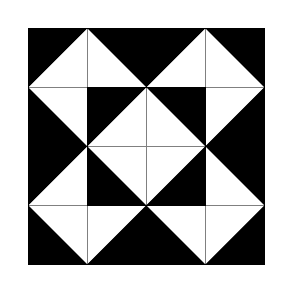
\begin{tikzpicture}[scale=0.75]
 \draw [step=1cm,gray,very thin](0,-1) grid (4,3); 
 \draw[opacity=1,fill=black](1,-1)--(0,-1)--(0,0); 
 \draw[opacity=1,fill=black](0,0)--(0,1)--(1,1); 
 \draw[opacity=1,fill=black](1,1)--(0,1)--(0,2); 
 \draw[opacity=1,fill=black](0,2)--(0,3)--(1,3); 
 \draw[opacity=1,fill=black](2,0)--(2,-1)--(1,-1); 
 \draw[opacity=1,fill=black](2,0)--(1,0)--(1,1); 
 \draw[opacity=1,fill=black](1,1)--(1,2)--(2,2); 
 \draw[opacity=1,fill=black](1,3)--(2,3)--(2,2); 
 \draw[opacity=1,fill=black](3,-1)--(2,-1)--(2,0); 
 \draw[opacity=1,fill=black](3,1)--(3,0)--(2,0); 
 \draw[opacity=1,fill=black](2,2)--(3,2)--(3,1); 
 \draw[opacity=1,fill=black](2,2)--(2,3)--(3,3); 
 \draw[opacity=1,fill=black](4,0)--(4,-1)--(3,-1); 
 \draw[opacity=1,fill=black](3,1)--(4,1)--(4,0); 
 \draw[opacity=1,fill=black](4,2)--(4,1)--(3,1); 
 \draw[opacity=1,fill=black](3,3)--(4,3)--(4,2); 
\end{tikzpicture} 
 & 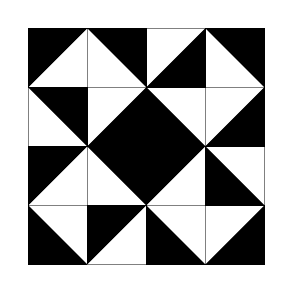
\begin{tikzpicture}[scale=0.75]
 \draw [step=1cm,gray,very thin](0,-1) grid (4,3); 
 \draw[opacity=1,fill=black](1,-1)--(0,-1)--(0,0); 
 \draw[opacity=1,fill=black](0,0)--(0,1)--(1,1); 
 \draw[opacity=1,fill=black](0,2)--(1,2)--(1,1); 
 \draw[opacity=1,fill=black](0,2)--(0,3)--(1,3); 
 \draw[opacity=1,fill=black](1,-1)--(1,0)--(2,0); 
 \draw[opacity=1,fill=black](1,1)--(2,1)--(2,0); 
 \draw[opacity=1,fill=black](2,2)--(2,1)--(1,1); 
 \draw[opacity=1,fill=black](1,3)--(2,3)--(2,2); 
 \draw[opacity=1,fill=black](3,-1)--(2,-1)--(2,0); 
 \draw[opacity=1,fill=black](2,0)--(2,1)--(3,1); 
 \draw[opacity=1,fill=black](3,1)--(2,1)--(2,2); 
 \draw[opacity=1,fill=black](3,3)--(3,2)--(2,2); 
 \draw[opacity=1,fill=black](4,0)--(4,-1)--(3,-1); 
 \draw[opacity=1,fill=black](4,0)--(3,0)--(3,1); 
 \draw[opacity=1,fill=black](4,2)--(4,1)--(3,1); 
 \draw[opacity=1,fill=black](3,3)--(4,3)--(4,2); 
\end{tikzpicture} 
 & 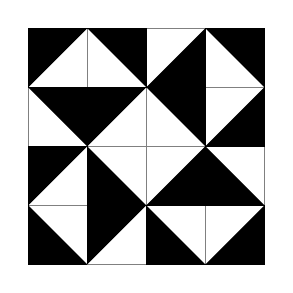
\begin{tikzpicture}[scale=0.75]
 \draw [step=1cm,gray,very thin](0,-1) grid (4,3); 
 \draw[opacity=1,fill=black](1,-1)--(0,-1)--(0,0); 
 \draw[opacity=1,fill=black](0,0)--(0,1)--(1,1); 
 \draw[opacity=1,fill=black](0,2)--(1,2)--(1,1); 
 \draw[opacity=1,fill=black](0,2)--(0,3)--(1,3); 
 \draw[opacity=1,fill=black](1,-1)--(1,0)--(2,0); 
 \draw[opacity=1,fill=black](2,0)--(1,0)--(1,1); 
 \draw[opacity=1,fill=black](1,1)--(1,2)--(2,2); 
 \draw[opacity=1,fill=black](1,3)--(2,3)--(2,2); 
 \draw[opacity=1,fill=black](3,-1)--(2,-1)--(2,0); 
 \draw[opacity=1,fill=black](3,1)--(3,0)--(2,0); 
 \draw[opacity=1,fill=black](2,2)--(3,2)--(3,1); 
 \draw[opacity=1,fill=black](3,3)--(3,2)--(2,2); 
 \draw[opacity=1,fill=black](4,0)--(4,-1)--(3,-1); 
 \draw[opacity=1,fill=black](4,0)--(3,0)--(3,1); 
 \draw[opacity=1,fill=black](4,2)--(4,1)--(3,1); 
 \draw[opacity=1,fill=black](3,3)--(4,3)--(4,2); 
\end{tikzpicture} 
\\ 
 \end{tabular} 
\marginnote{[object Object]}
\end{center}

\newpage

